% !TEX root = ../prj4projektdokumentation.tex
% SKAL STÅ I TOPPEN AF ALLE FILER FOR AT MASTER-filen KOMPILERES 

\chapter{Projektbeskrivelse}

Formålet med dette projekt, er at opbygge et system, der simulerer det danske transmissionssystem. For energileverandører i Danmark er det et lovmæssigt krav, at spændingsforsyningen hos forbrugerne altid ligger på 230 volt $\pm$10 procent, og det ønskes at undersøge mulighederne for at opfylde dette.\\ 
I dette projekt vil fokus være på stykket fra distributionstransformer og ud til forbrugere/belastninger. Systemet skal bestå af en spændingsregulator (trinkobler), en distributionslinje og to eller flere varierende belastninger. Det ønskes at måle strøm, spænding, power factor og effektretning således, at spændingsregulatoren hele tiden kan holde spændingen på $\pm$ et givent niveau, selvom belastningen ændres. Normalt måles disse værdier ved distributionstransformeren, men i dette projekt ønskes det at måle hos hver enkelt belastning. På den måde fås en bedre overvågning af systemet og bedre mulighed for at observere hvilken betydning, f.eks. belastningens afstand til distributionstransformeren har for spændingsniveauet.\\ Systemet skal have to indstillinger – en til manuelt valg af spændingsniveau og en til automatisk valg af passende spændingsniveau.\\ 
Det ønskes desuden at kunne måle frekvensindholdet i systemet for at kunne observere et eventuelt indhold af harmoniske. De harmoniske i systemet er højfrekvente og vil afsætte varme i transformerne og dermed forkorte deres levetid. Det er derfor relevant at kende til indholdet af disse.\\ 
Det er et krav, at målte værdier i systemet vises på en skærm. 

\begin{figure}[htbp] % (alternativt [H])
	\centering
	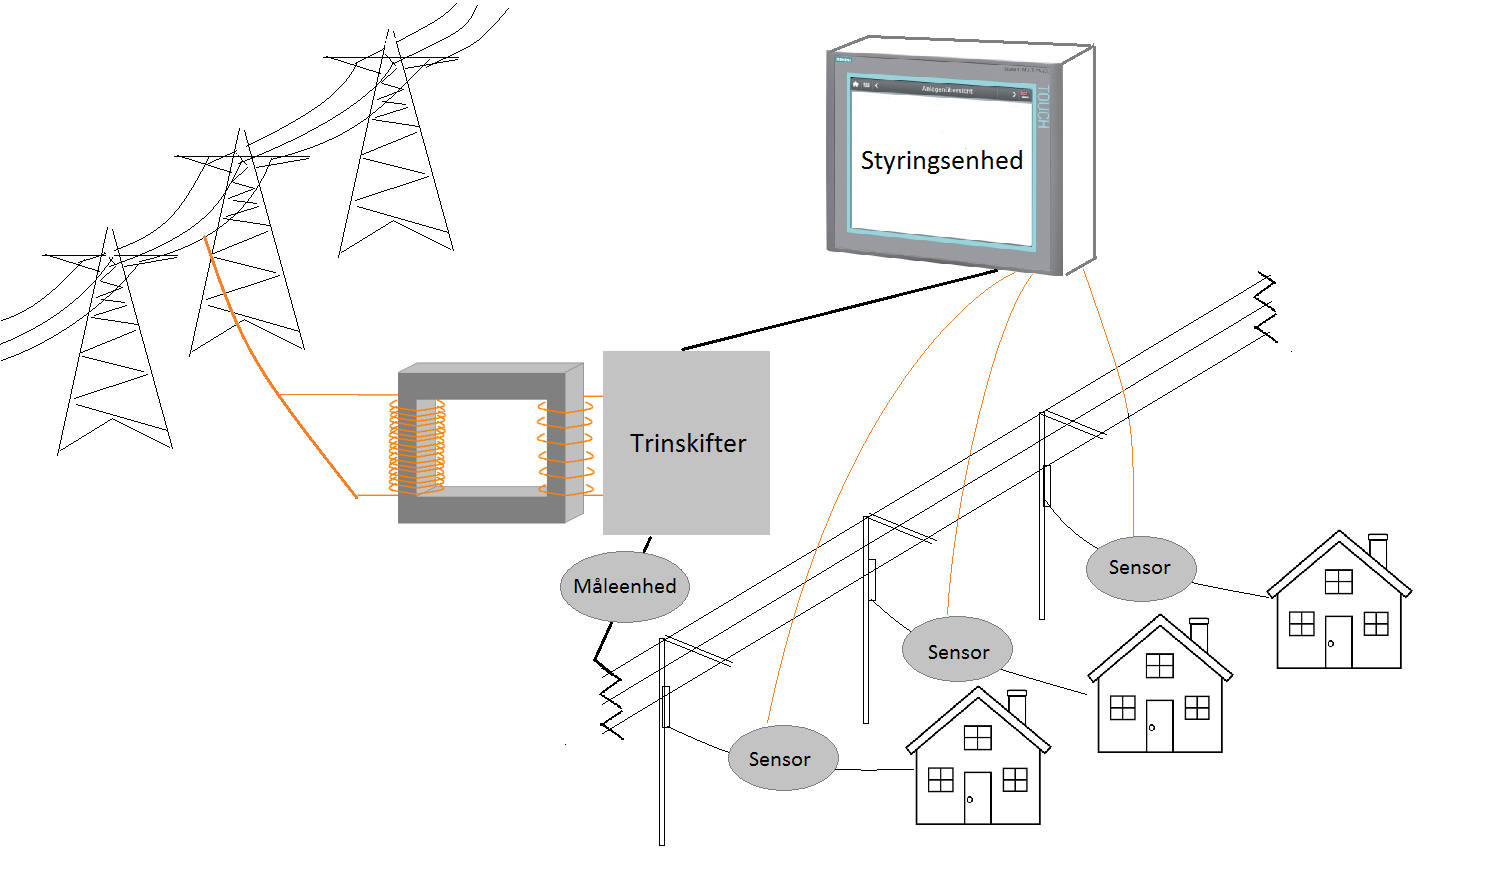
\includegraphics[width=0.7\textwidth]{Figure/RigtBillede}
	\caption{Visuel fremvisning af system}
	\label{fig:Rigtbillede}
\end{figure}